\documentclass{article}
\usepackage{float}
\usepackage[margin = 2cm]{geometry}
\usepackage{graphicx}
\usepackage{bm}
\usepackage{amsmath,amssymb,amsfonts,amsthm}
\setlength{\parindent}{0pt}

\newcommand{\spacer}[1][8pt]{
    \par\vspace{#1}
}

\author
{
    Mattia Boscolo Meneguolo - 2066700, \\
    Matteo Cuzzolin - 2066701
}
\title{Tesina di Fondamenti di Controlli Automatici, A.A. 2024}
\date{}
\begin{document}
\maketitle

\begin{figure}[!htbp]
    \centering
    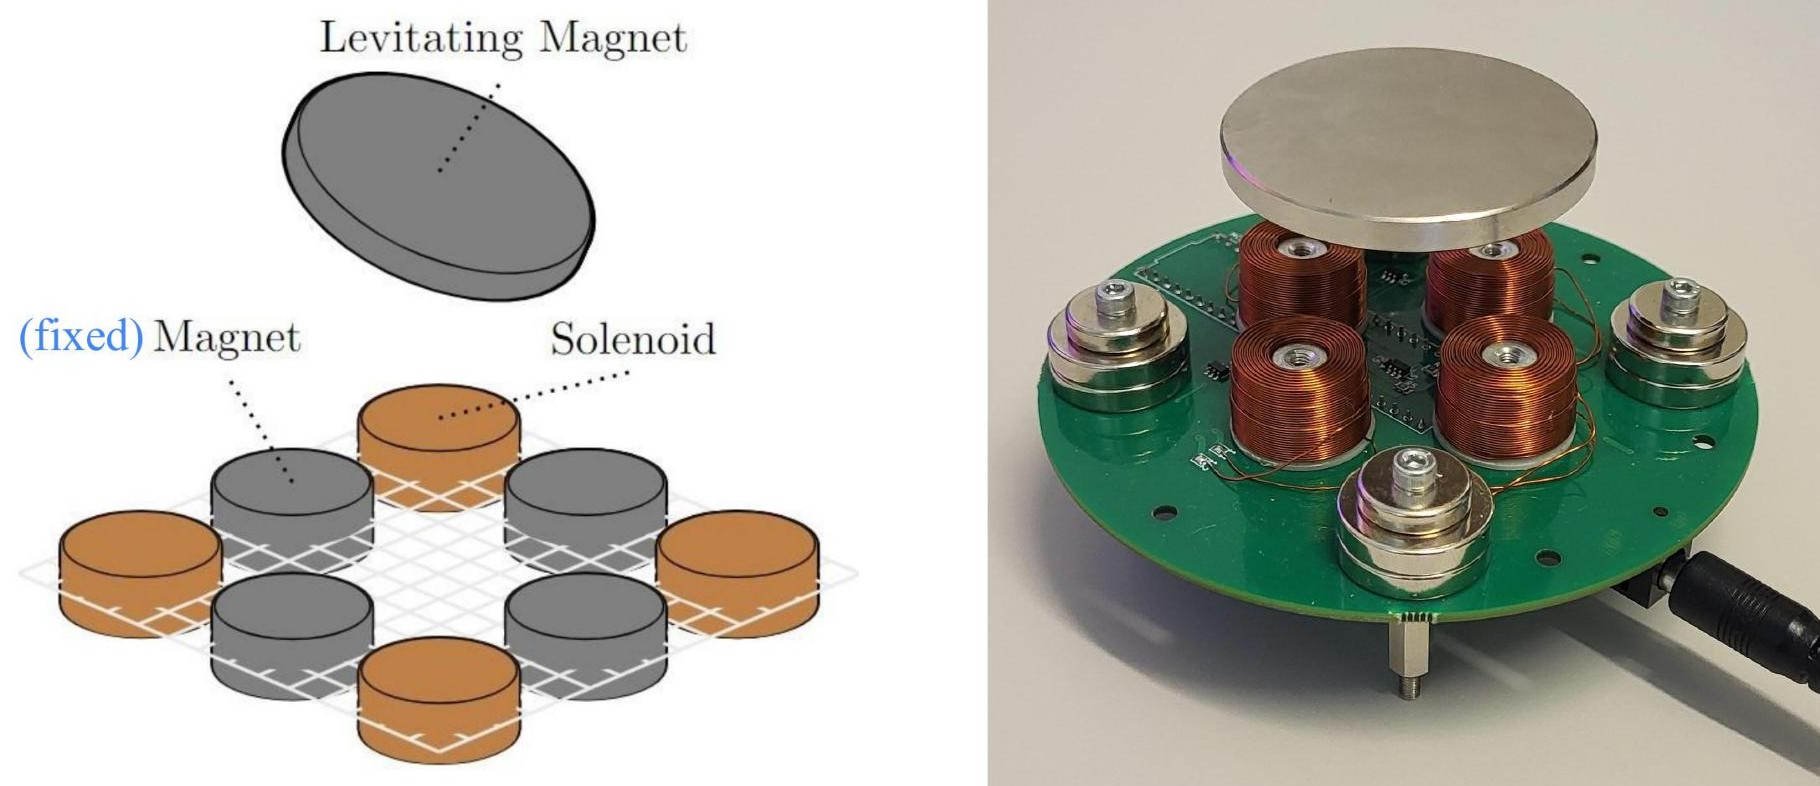
\includegraphics[width = 0.8\textwidth]{Images/maglev-system-schematics}
    \caption{Rappresentazione del sistema - Implementazione del sistema}
    \label{fig:rappresentazione_sistema}
\end{figure}

Sia $\tilde{z}(t) = z(t) - \overline{z}$ dove $z(t)$ è la posizione del magnete e $\overline{z}$ è la posizione del magnete all'equilibrio.

La trasformata di laplace di $\tilde{z}$ è:
$$\tilde{Z}(s) = \frac{b_s}{\overline{z}ms^2+\overline{z}ds+mg}I(s)+\frac{(ms+d)\tilde{z}(0)+m\tilde{z}'(0)}{ms^2+ds+\frac{mg}{\overline{z}}}$$

\section{Esercizio 1}
Studiamo la risposta libera, infatti in questo caso $i(t) = 0 \:\forall t$. Ipotizziamo anche che $\tilde{z}'(0) = 0$

$\tilde{Z}(s) =\frac{(ms+d)\tilde{z}(0)}{ms^2+ds+\frac{mg}{\overline{z}}}$

\spacer
Secondo la regola di Cartesio il polinomio al denominatore è stabile infatti tutti i coefficienti sono non nulli e positivi.

\spacer
Tuttavia dalle prime elaborazioni su mathlab risulta evidente che il sistema impiega un lungo periodo di tempo per assestarsi alla posizione di equilibrio.
Dato che vogliamo svolgere diverse simulazioni per mostrare che il sistema raggiunge l'equilibrio al variare di $\tilde{z}(0)$ aumenteremo il valore di d a 0.1 così da rendere più veloci le simulazioni.

\spacer
Questo è un esempio di una simulazione con $\tilde{z}(0)=0.35$ e $d=0.1$

\begin{figure}[H]
    \centering
    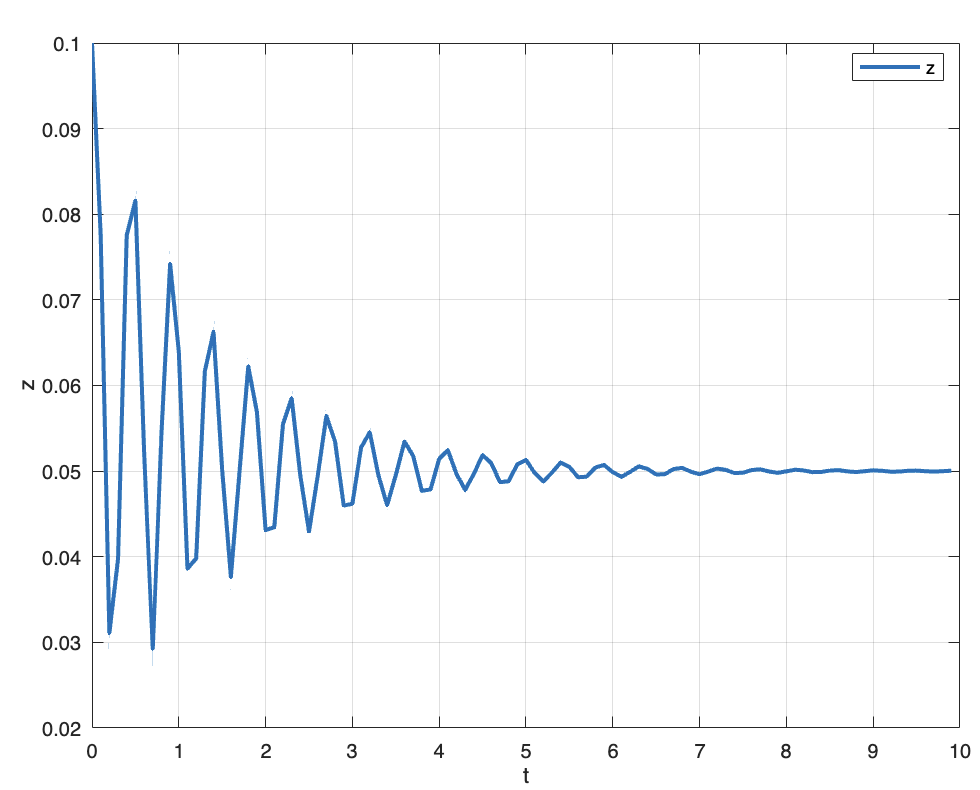
\includegraphics[width = 0.5\textwidth]{Images/simulazione-d-0.1.png}
    \caption{Simulazione $\tilde{z}(0)=0.35$}
    \label{fig:simulazione_d_0.1}
\end{figure}

\spacer
A questo punto simuliamo il sistema al variare di $\tilde{z}(0)$ e verifichiamo che dopo 10 secondi esso si assesti all'altezza di equilibrio.

\begin{figure}[H]
    \centering
    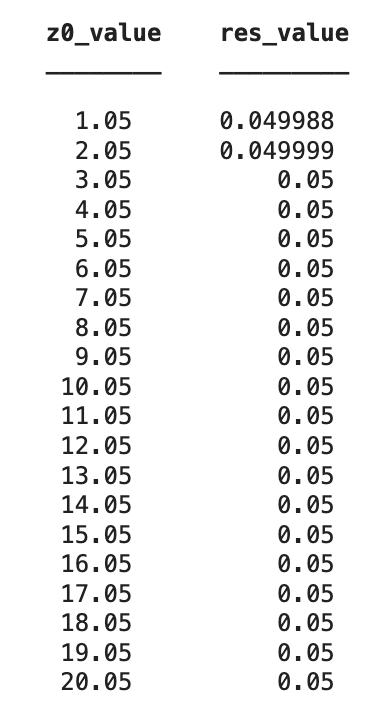
\includegraphics[width = 0.2\textwidth]{Images/risultati-simulazioni.png}
    \caption{Simulazione $\tilde{z}(0) variabile$}
    \label{fig:simulazione_z_variabile}
\end{figure}

\section{Esercizio 2}
Vogliamo disegnare il luogo delle radici della funzione di trasferimento in catena aperta del sistema, per fare questo usiamo mathlab e otteniamo:

\begin{figure}[H]
    \centering
    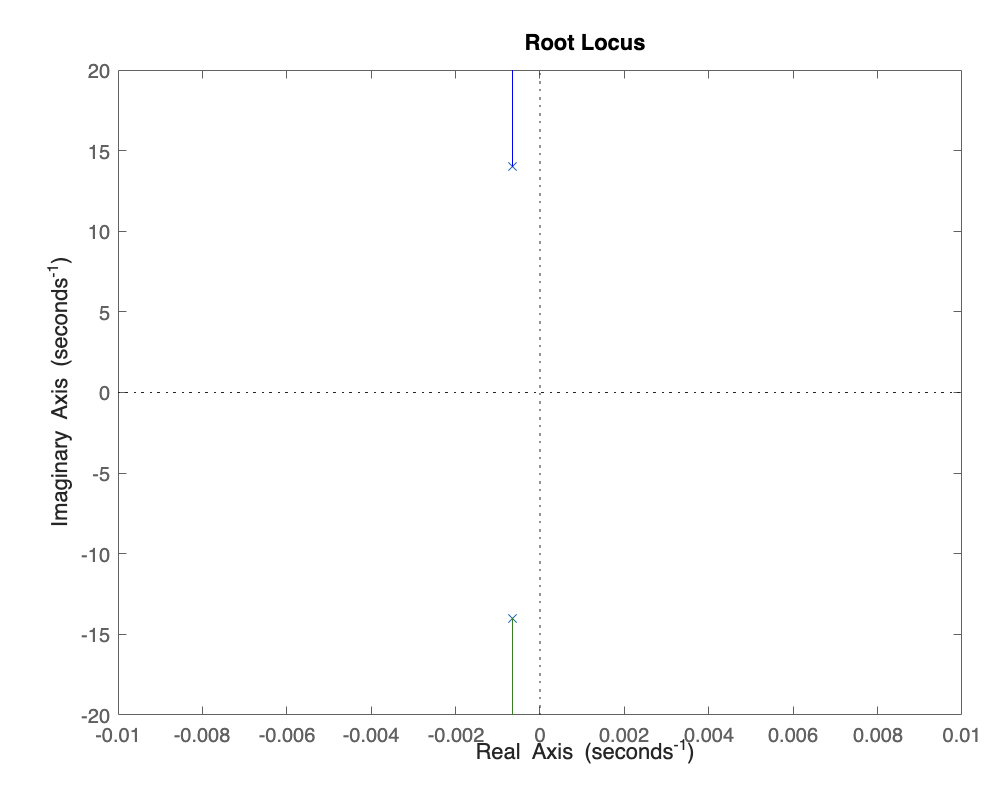
\includegraphics[width = 0.5\textwidth]{Images/luogo-radici-proporzionale.png}
    \caption{Luogo Radice in catena aperta}
    \label{fig:luogo_radice_catena_aperta}
\end{figure}

Per ottenere un controllore con un tempo di salita $T_s \le 1$ vogliamo $T_s = \frac{2}{w_n} \Rightarrow w_n = |p| = 2$

Ma le radici più vicine all'origine hanno $|p| = 14.0071$

Non è quindi possibile costruire un controllore proporzionale con i requisiti richiesti.

\section{Esercizio 3}
Scegliamo come indici di performace quelli richiesti dall'esercizio precedente, ovvero 1 secondo di settling time, quindi anche il tempo di salita deve essere inferiore al secondo.
Inoltre cerchiamo un controllore che abbia la minima sovraelongazione.

\spacer
Abbiamo prima utilizzato un noto metodo euristico, detto Ziegler-Nichols. Seguendo il semplice algoritmo abbiamo ottenuto i seguenti valori del controllore:

$K_p = 8.4028;$

$K_i = 10.1198;$

$K_d = 0.37896;$

\spacer
Ottenendo così il seguente risultato:

\begin{figure}[H]
    \centering
    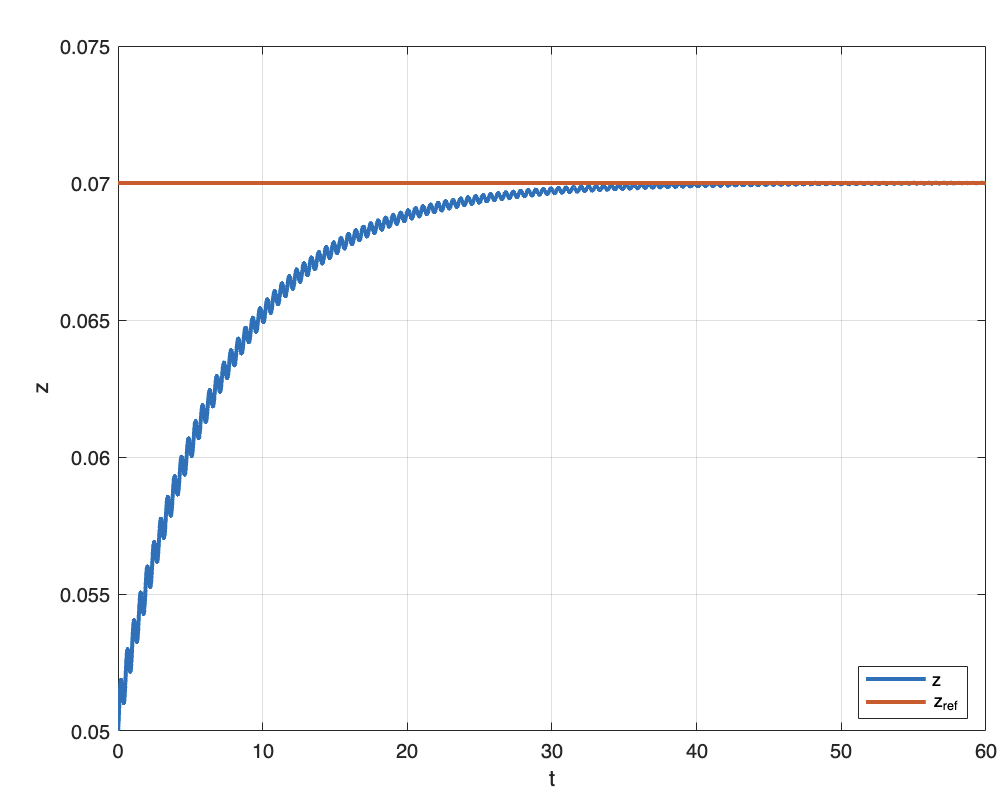
\includegraphics[width = 0.5\textwidth]{Images/PID-euristico.png}
    \caption{Sistema controllato con PID ottenuto con il metodo Ziegler-Nichols}
    \label{fig:Ziegler_Nichols_PID}
\end{figure}

Questo controllore non soddisfa le nostre richieste in quanto impiega circa 40 secondi a raggiungere il regime, tuttavia non presenta alcuna sovraelongazione.

\spacer
Per trovare un controllore con prestazioni migliori abbiamo utilizzato la funzione \texttt{pidTuner} di Mathlab.

Utilizzando i valori restituiti dal tuner, ovvero:

$K_p = 8.9131;$

$K_i = 52.4269;$

$K_d = 0.37883;$

\spacer
Ottenendo così il seguente risultato:

\begin{figure}[H]
    \centering
    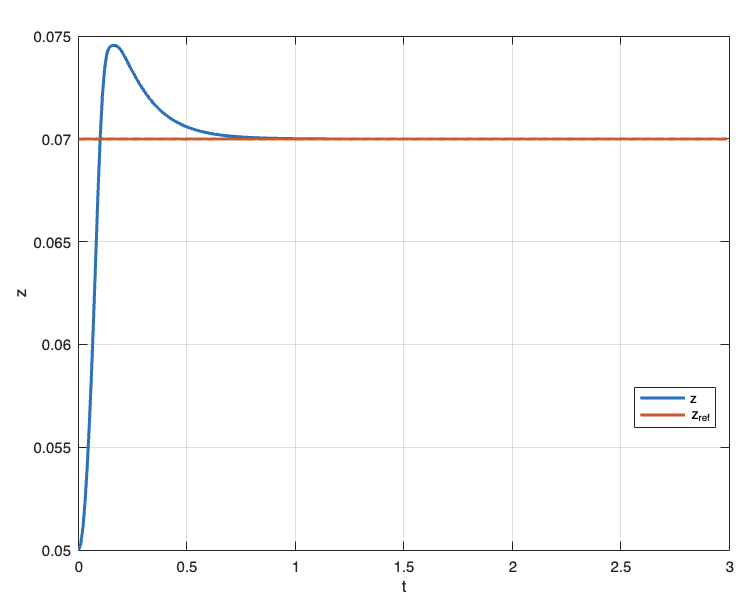
\includegraphics[width = 0.5\textwidth]{Images/PID-tuner.png}
    \caption{Sistema controllato con PID ottenuto con pidTuner}
    \label{fig:pidTuner-PID}
\end{figure}

Il controllore ottenuto è di gran lunga migliore e soddisfa i requisiti che ci eravamo posti, porta il sistema a regime in poco meno di un secondo tuttavia ha una sovraelongazione importante.

\spacer
Infine abbiamo voluto cercare un controllore con una minore sovraelongazione, ignorando il limite di tempo.

Utilizzando i seguenti valori:

$K_p = 7.2786;$

$K_i = 14.8316;$

$K_d = 0.89298;$

\spacer
Ottenendo così il seguente risultato:

\begin{figure}[H]
    \centering
    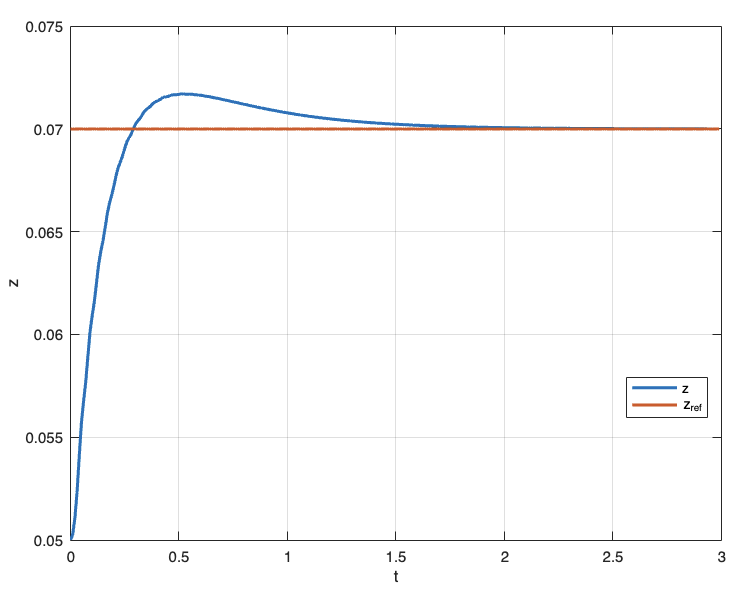
\includegraphics[width = 0.5\textwidth]{Images/PID-tuner-overshoot.png}
    \caption{Sistema controllato con PID ottenuto con pidTuner con richieste modificate}
    \label{fig:pidTuner-PID-overshoot}
\end{figure}

\section{Esercizio 4}
Per verificare l'altezza massima che il magnete è in grado di raggiungere impostiamo i solenoidi alla massima potenza a loro disponibile, ovvero $i = 0.02$.

Per velocizzare la simulazione ed ottenere il valore finale in un tempo minore abbiamo aumentato l'attrito impostando $d = 0.1$.

\begin{figure}[H]
    \centering
    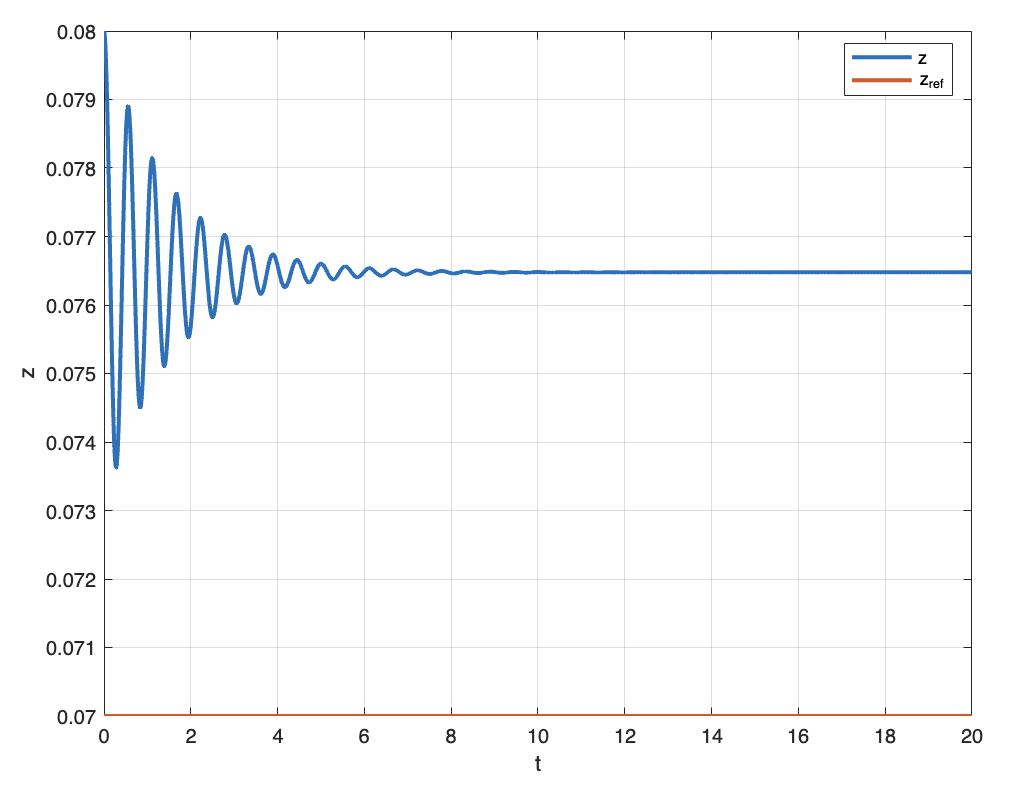
\includegraphics[width = 0.5\textwidth]{Images/max-z.png}
    \caption{Sistema controllato con i = 0.02}
    \label{fig:max-z}
\end{figure}

Vediamo sperimentalmente che il valore massimo a regime che il sistema può raggiungere è $0.0764771$.

\section{Esercizio 5}
Per far seguire al magnete i segnali di riferimento richiesti abbiamo utilizzato in entrambi i casi un controllore PID con valori modificati per adattarsi meglio al problema.

\spacer
Nel caso del riferimento sinusoidale abbiamo utilizzato il controllore fornito dal tuner di mathlab:

$K_p = 8.9131;$

$K_i = 52.4269;$

$K_d = 0.37883;$

\begin{figure}[H]
    \centering
    \begin{minipage}{0.45\textwidth}
        \begin{figure}[H]
            \centering
            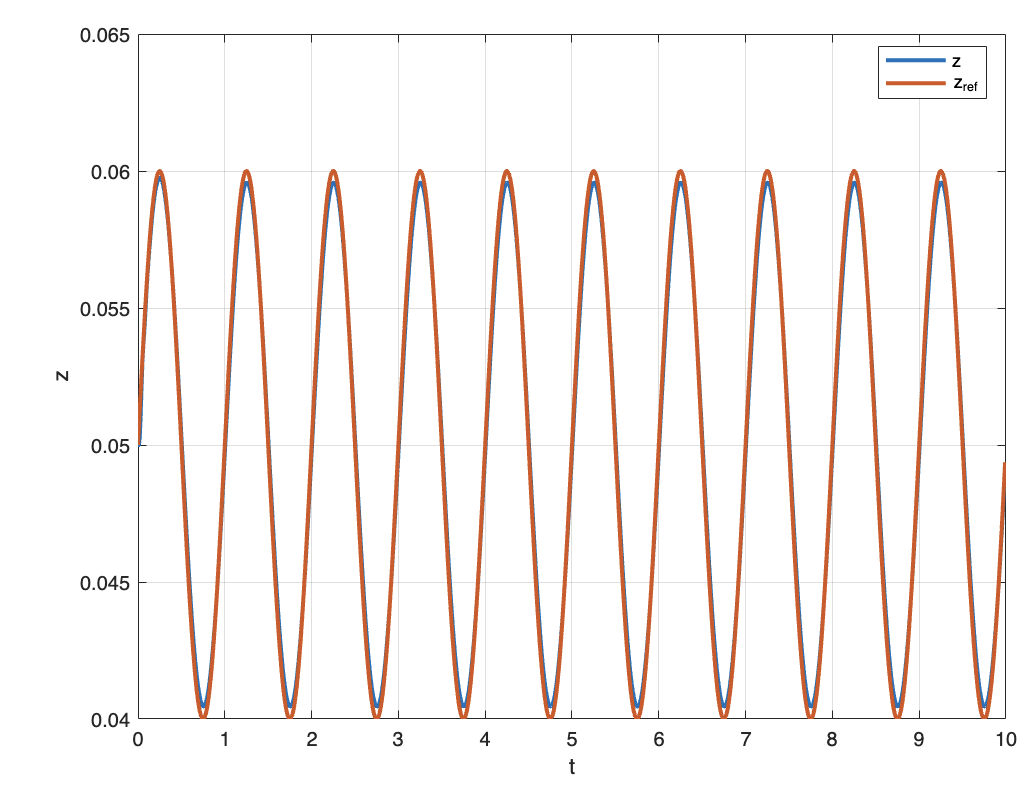
\includegraphics[width = 1\textwidth]{Images/sine.png}
            \caption{Sistema controllato con controllore PID}
            \label{fig:PID-sine}
        \end{figure}
    \end{minipage}
    \hfill
    \begin{minipage}{0.45\textwidth}
        \begin{figure}[H]
            \centering
            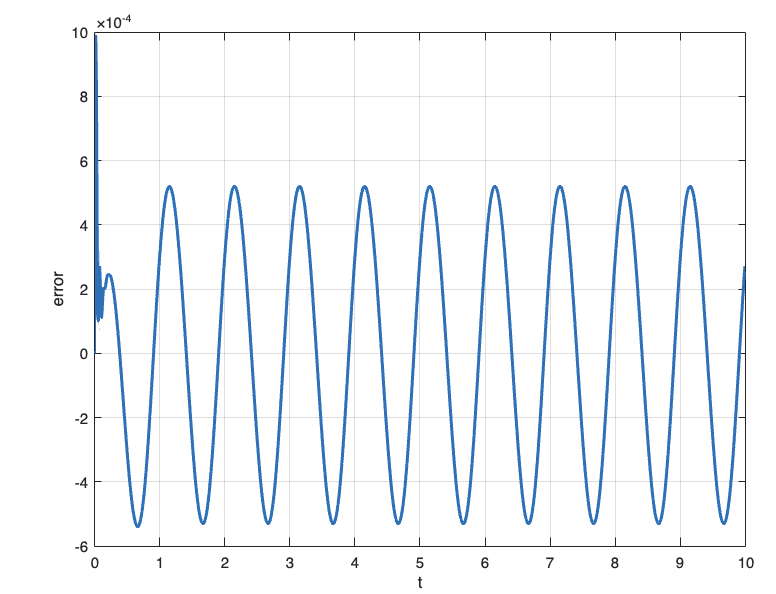
\includegraphics[width = 1\textwidth]{Images/sine-error.png}
            \caption{Errore del sistema}
            \label{fig:PID-sine-error}
        \end{figure}
    \end{minipage}
\end{figure}

\spacer
Nel caso del riferimento ad onda quadra abbiamo utilizzato dei valori forniti dal tuner, ma leggermente modificati:

$K_p = 8.4028;$

$K_i = 10.1198;$

$K_d = 0.37896;$

\begin{figure}[H]
    \centering
    \begin{minipage}{0.45\textwidth}
        \begin{figure}[H]
            \centering
            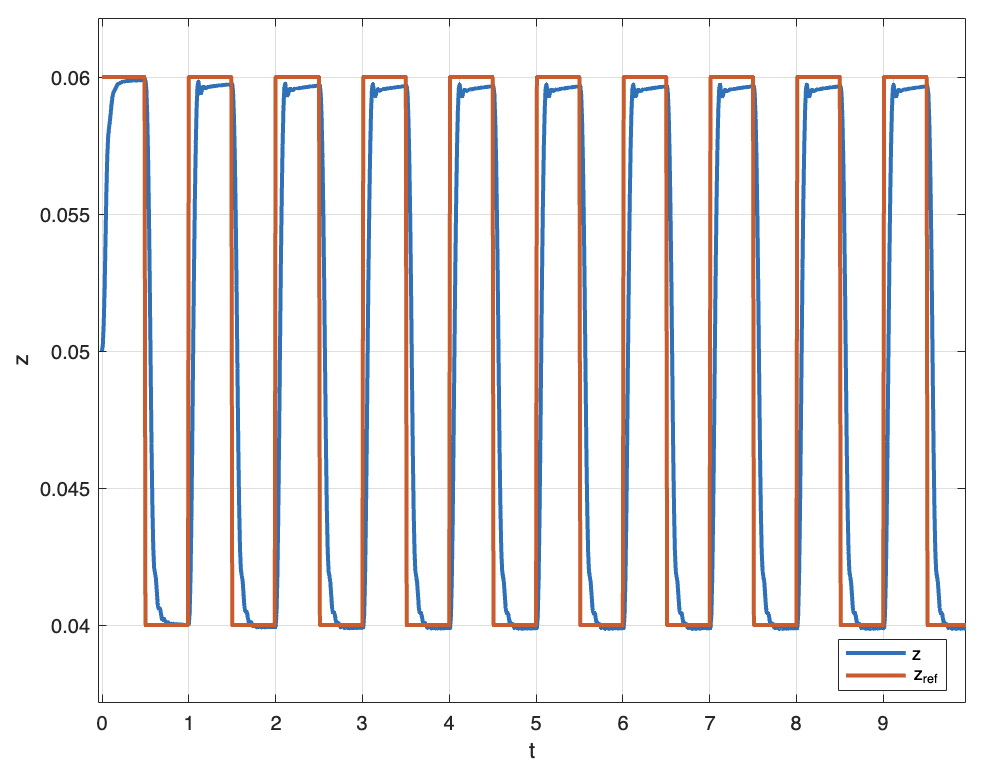
\includegraphics[width = 1\textwidth]{Images/square.png}
            \caption{Sistema controllato con controllore PID}
            \label{fig:PID-square}
        \end{figure}
    \end{minipage}
    \hfill
    \begin{minipage}{0.45\textwidth}
        \begin{figure}[H]
            \centering
            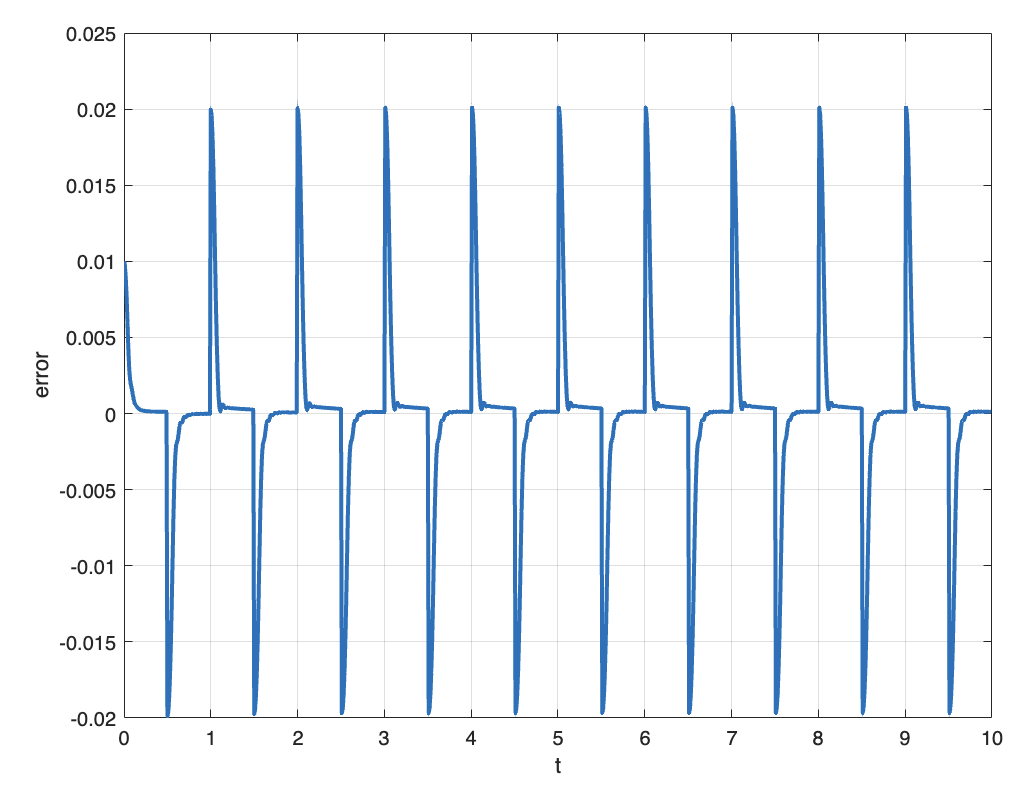
\includegraphics[width = 1\textwidth]{Images/square-error.png}
            \caption{Errore del sistema}
            \label{fig:PID-square-error}
        \end{figure}
    \end{minipage}
\end{figure}

In entrambi i casi il magnete segue accuratamente il segnale di riferimento, all'interno dei requisiti posti dal problema.

\end{document}
